
\section{Impact of pile-up}

\label{sec:pileup}

The discussion so far has not accounted for the effects of
pile-up (PU), which are known to be very important at the HL-LHC.
%
In this section, we show how our qualitative results, in particular
the enhanced discrimination provided by the MVA, are robust
in the presence of realistic PU conditions.


First of all we describe the simulation of realistic
PU conditions at the HL-LHC, and discuss the settings of
the PU subtraction strategy that we adopt.
%
Then we present the validation of the PU subtraction,
and compare a number of distributions, including substructure variables,
with and without PU.
%
Finally we revisit the MVA analysis of Sect.~\ref{sec:mva}, and
show that our qualitative conclusions are robust
in the presence of realistic PU conditions.
%
As we will show now, a signal significance for
Higgs production in the $4b$ final state
of up to $S/\sqrt{B}\simeq 4$
can be achieved at the HL-LHC even accounting for PU.


\subsection{PU subtraction with {\tt SoftKiller}}

To study the impact of PU in our analysis,
a large number
of Minimum Bias (MB) events,
including Multiple Parton Interactions (MPI),
have been added to the signal
and background samples described in Sect.~\ref{mcgeneration}.
%
We have explored two scenarios for the amount of PU expected
at the HL-LHC, one with a mean number of
PU vertices of $\la n_{\rm PU}\ra=80$, and another
with $\la n_{\rm PU}\ra=150$.
%
MB events have been generated with {\tt Pythia8} using
the Monash 2013 tune.
%
We have generated a total of 100M minimum-bias events, which are
then randomly superimposed to the hard-scattering events.

In order to subtract the PU, a large number of techniques
have been proposed recently~\cite{Cacciari:2009dp,TheATLAScollaboration:2013pia,Butterworth:2008iy,Cacciari:2007fd,Krohn:2009th,Krohn:2013lba,Ellis:2009me,Bertolini:2014bba,Cacciari:2014gra,Cacciari:2014jta,Berta:2014eza,Larkoski:2014wba}.
%
In this work, PU  will be subtracted by means
of the the {\tt SoftKiller}
method~\cite{Cacciari:2014gra}, as implemented in {\tt FastJet}.
%
Let us note however that
a systematic optimization of the PU subtraction strategy is beyond
the scope of this work, and in particular that further
improvements over the results presented below is feasible
with further tuning of the PU subtraction.


The idea underlying {\tt SoftKiller} is based on eliminating particles
below a given cut-off in their transverse momentum, $p_T^{\rm (cut)}$, whose
value is dynamically determined in a way that makes the event-wide
transverse-momentum flow density $\rho$ vanish.
%
This $p_T$ flow density is defined as
\be
\rho\equiv{\rm median}_i \Bigg\{ \frac{p_{Ti}}{A_i}\Bigg\} \, ,
\ee
where the median is computed over all the patches $i$ with area
$A_i$ and transverse momentum $p_{Ti}$ in which the $\lp \eta,\phi\rp$ plane
is partitioned.
%
From its definition, we observe that the value of $p_T^{(\rm cut)}$
will be dynamically raised until half of the patches have $\rho=0$.

The size and number of these patches is a free parameter of the algorithm -
here we will use square patched with length $a=0.4$.
%
We restrict ourselves to the central rapidity interval,
$\eta \in \lc -2.5, 2.5\rc$, for the estimation of the
$p_T$ flow density $\rho$, which is the region relevant
for the present analysis.
%
In this work, the {\tt SoftKiller} method is applied
to particles at the end of the parton shower, before
the jet clustering stage.

\subsection{Validation of the PU subtraction}

Now we turn to validate our PU subtraction strategy.
%
To this end, we compare different kinematical distributions
in the three relevant cases:
cases:
\begin{itemize}
\item without any PU,
\item adding PU, but without any PU subtraction,
  \item adding PU, followed by the {\tt SoftKiller} subtraction.
\end{itemize}
As we will show now, {\tt SoftKiller} exhibits a reasonable
performance in PU subtraction.
%
We will also see that the boosted category is less affected
by PU than the resolved category, as expected from the higher
$p_T$ threshold in the corresponding selection cuts.

Let us begin by comparing
a number of signal distributions with
and without PU, with $\la n_{\rm PU}\ra=80$ in the former
case.
%
In Fig.~\ref{fig:m_H_PU} we show the invariant mass distribution
of the leading and subleading Higgs candidates. in the boosted
and resolved categories.
%
These distributions are plotted after the $b$-tagging, that is,
before they are used as input to the MVA.
%
As we can see, in the boosted category, the residual effects of PU
after the {\tt SoftKiller} subtraction are very mild in these
distributions, with the position of the Higgs mass peaks essentially
unchanged.
%
The effects are more important for the resolved category, where PU
shifts the Higgs peak by an amount $\Delta m_h \simeq 5$ GeV.

%%%%%%%%%%%%%%%%%%%%%%%%
\begin{figure}[t]
  \begin{center}
      \vspace{-1cm}
      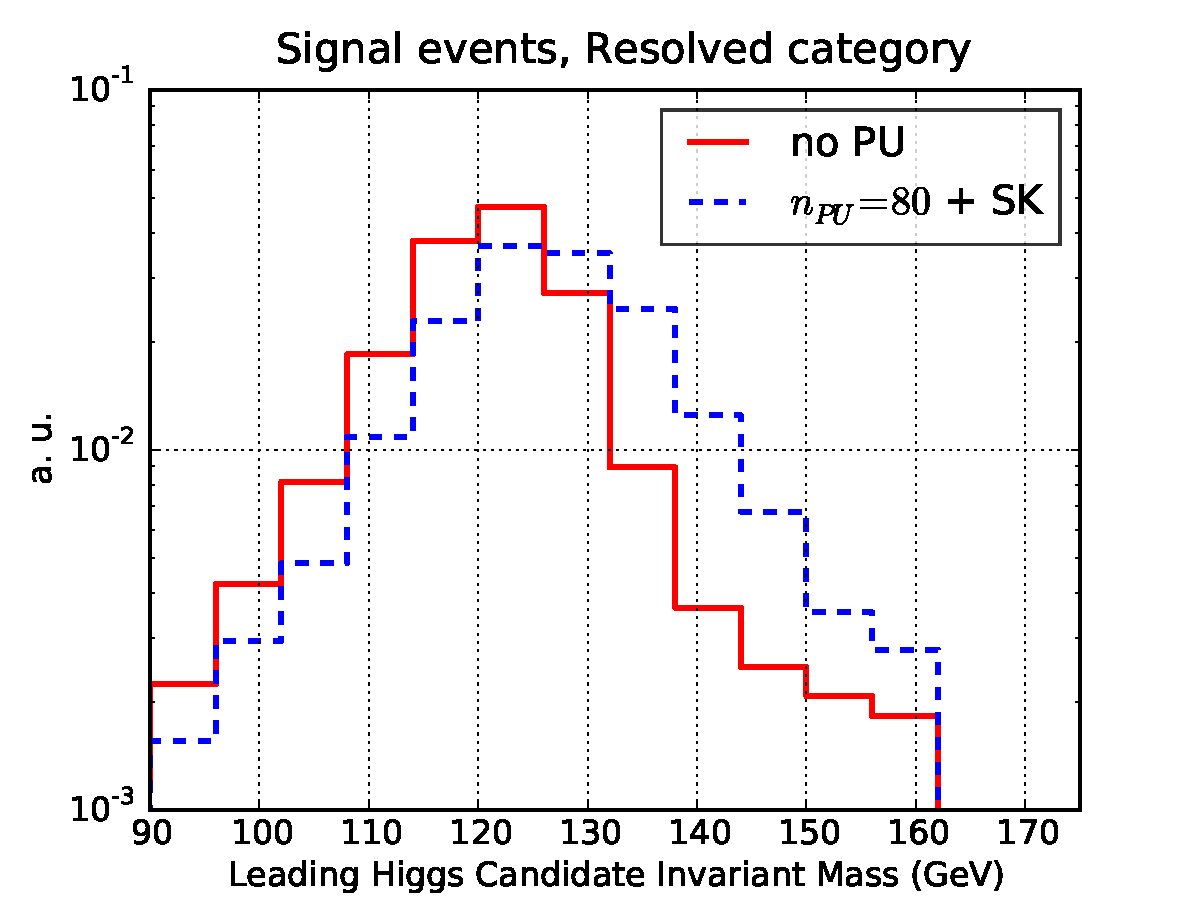
\includegraphics[width=0.49\textwidth]{plots/m_H0_res_comp.pdf}
      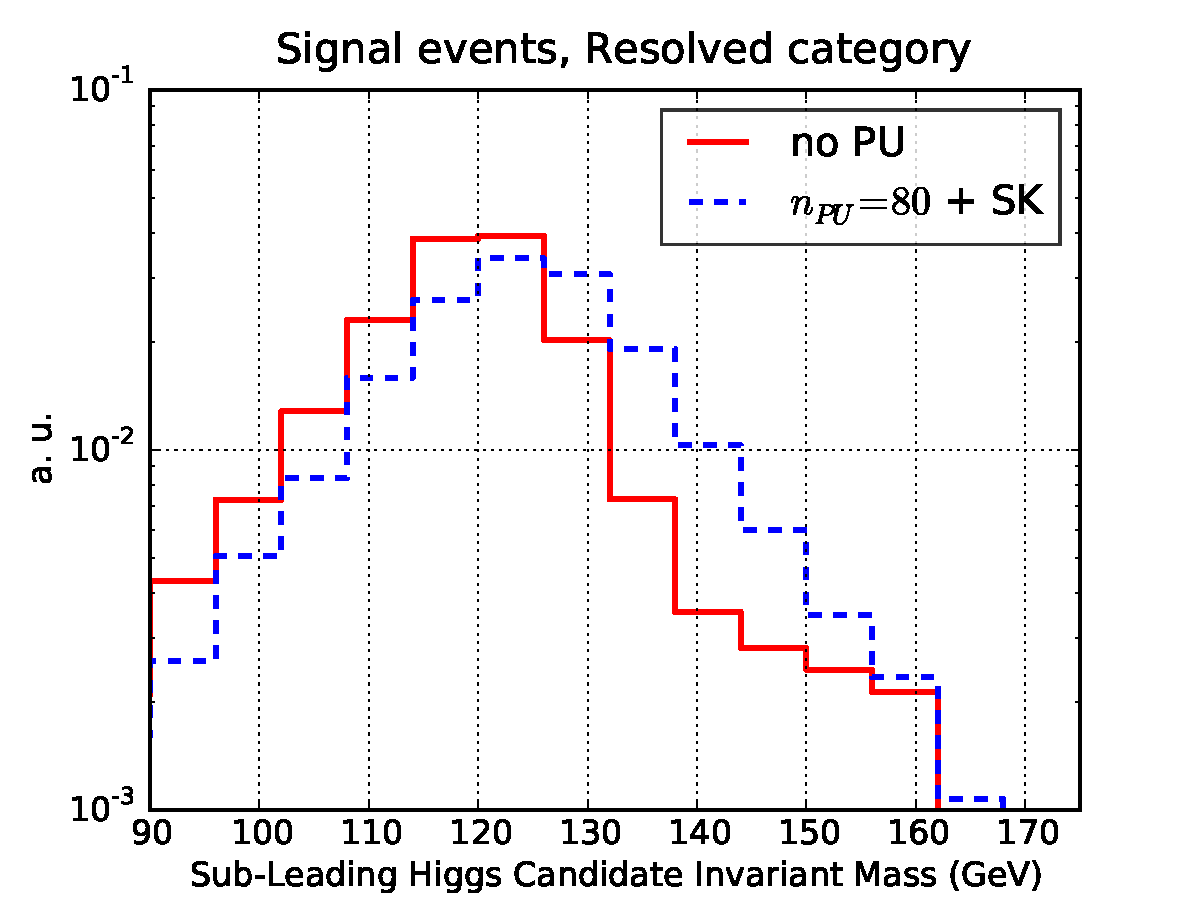
\includegraphics[width=0.49\textwidth]{plots/m_H1_res_comp.pdf}
      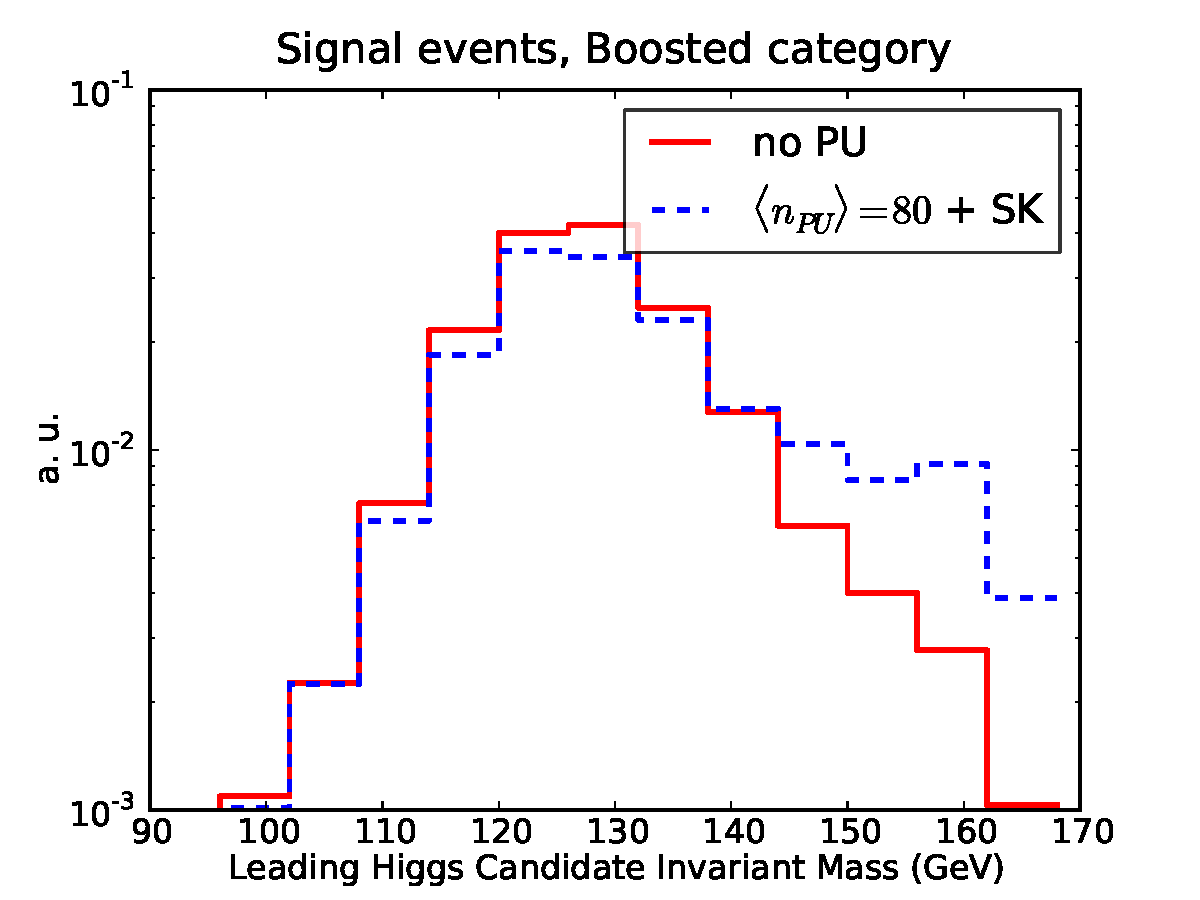
\includegraphics[width=0.49\textwidth]{plots/m_H0_bst_comp.pdf}
      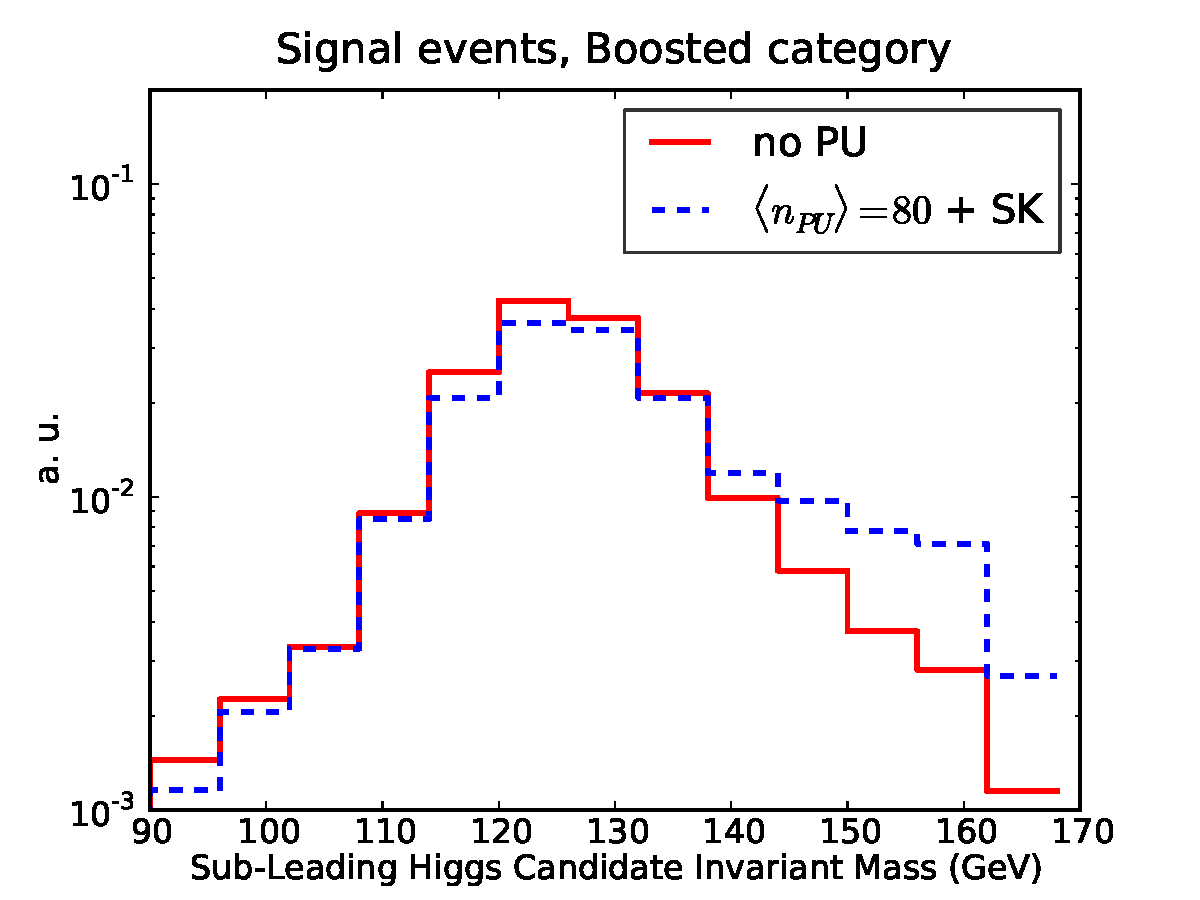
\includegraphics[width=0.49\textwidth]{plots/m_H1_bst_comp.pdf}
  \caption{\small
    Comparison of the invariant mass distributions of the leading (left plots)
    and subleading (right plots) Higgs candidates in the resolved
    (upper plots) and boosted (lower plots) categories,
    without PU and with $\la n_{PU}\ra=80$ subtracted with {\tt SoftKiller}.
}
\label{fig:m_H_PU}
\end{center}
\end{figure}
%%%%%%%%%%%%%%%%%%%%%%%

Next we compare the transverse momentum of the leading Higgs
candidate, $p_t^{h_1}$ and the invariant mass of the di-Higgs system
$m_{hh}$, in Fig.~\ref{fig:mHH_PU}, both for the boosted and
for the resolved categories.
%
In the case of the $p_T$, the differences between the resolved
and boosted selection cuts can be clearly observed.
%
The effect of PU is negligible in the boosted case, and small
in the resolved case, except for large $p_T$ values.
%
For the case of the $m_{hh}$ distribution, similar conclusions
apply.
%
Note that this latter observable is particularly sensitive
of BSM dynamics.


%%%%%%%%%%%%%%%%%%%%%%%%
\begin{figure}[t]
  \begin{center}
    \vspace{-1cm}
  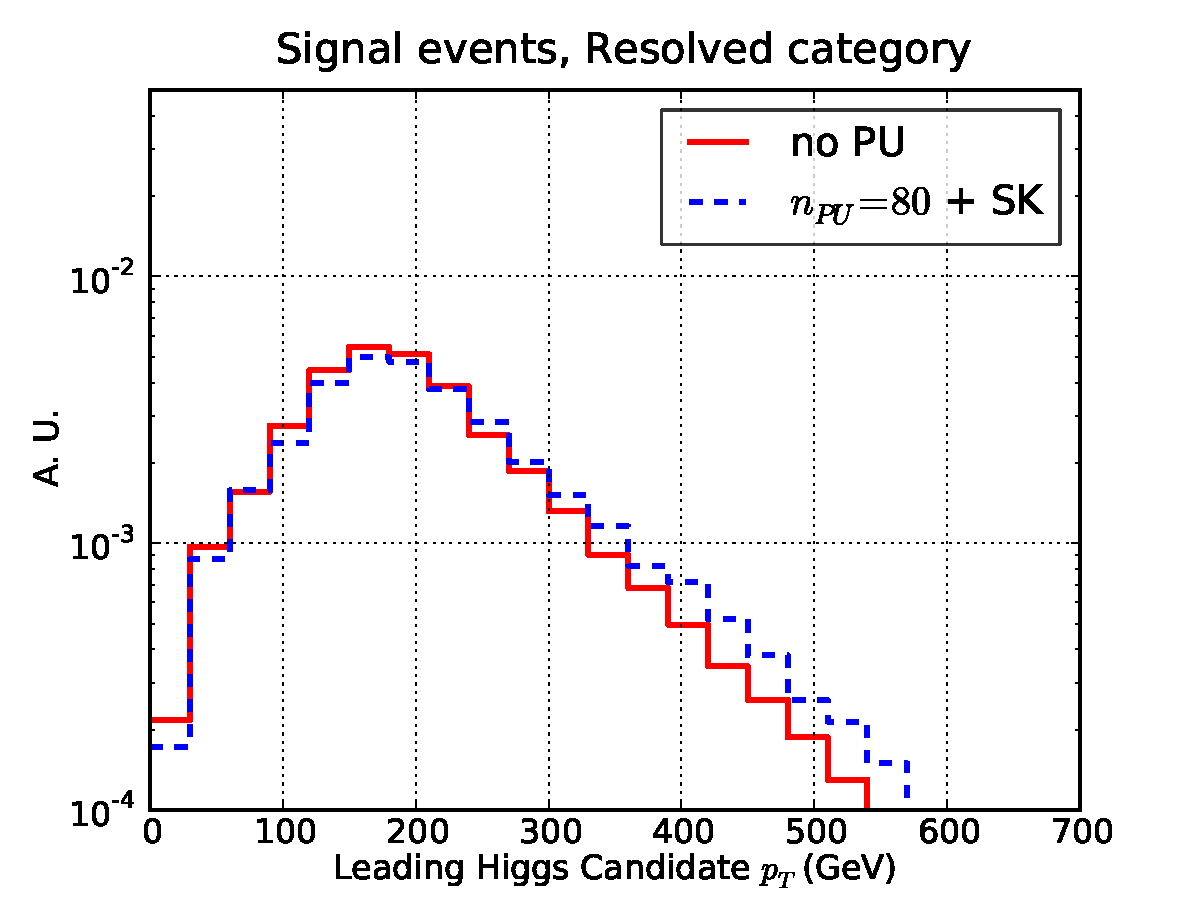
\includegraphics[width=0.49\textwidth]{plots/pt_H0_C2_res_comp.pdf}
  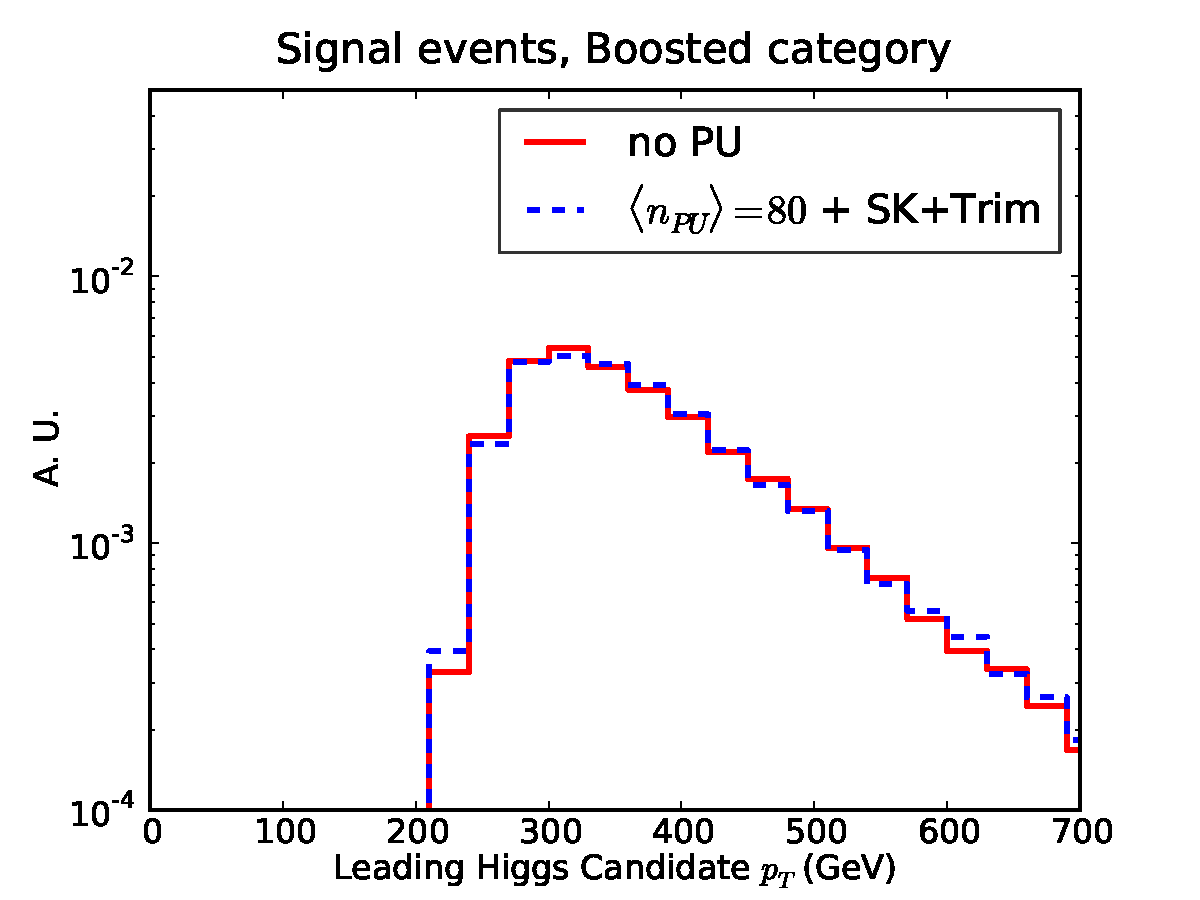
\includegraphics[width=0.49\textwidth]{plots/pt_H0_C2_bst_comp.pdf}
  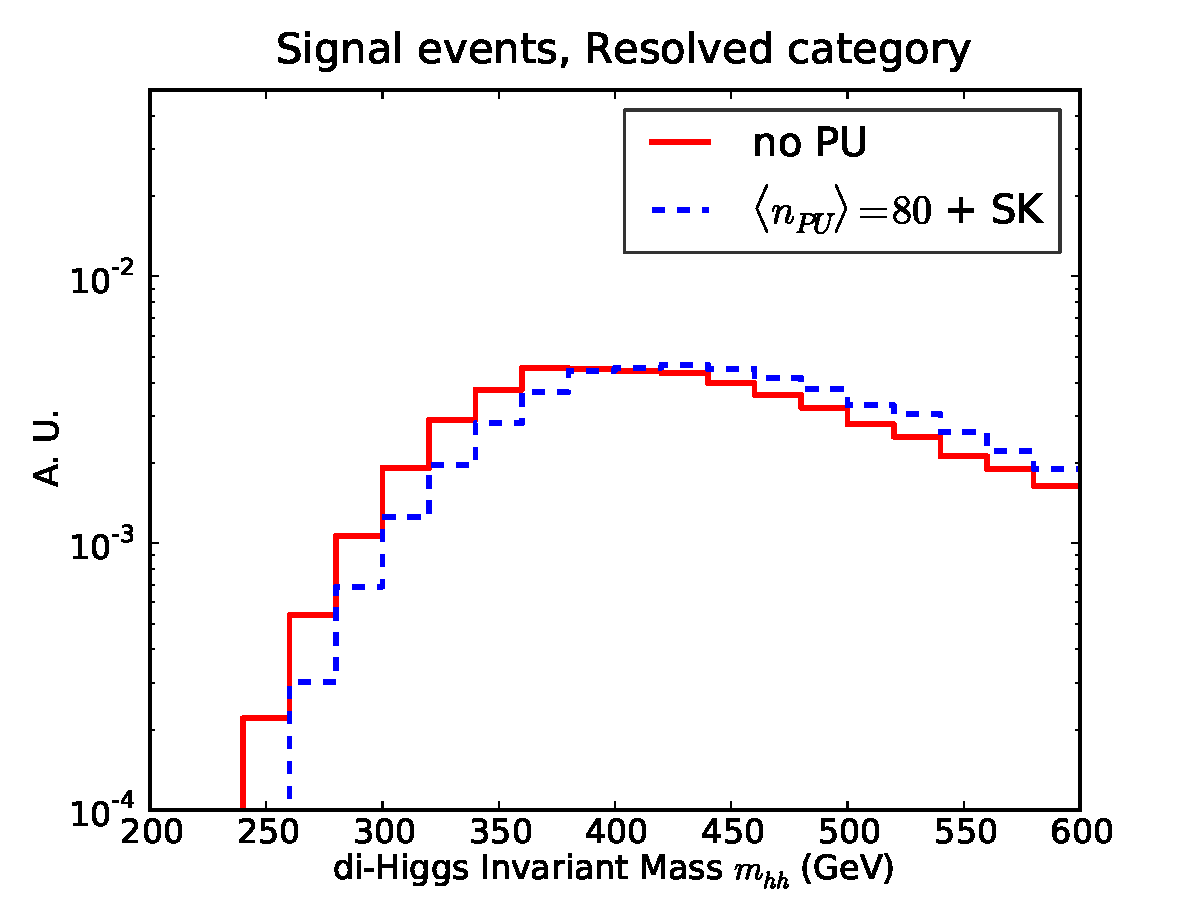
\includegraphics[width=0.49\textwidth]{plots/m_HH_C2_res_comp.pdf}
  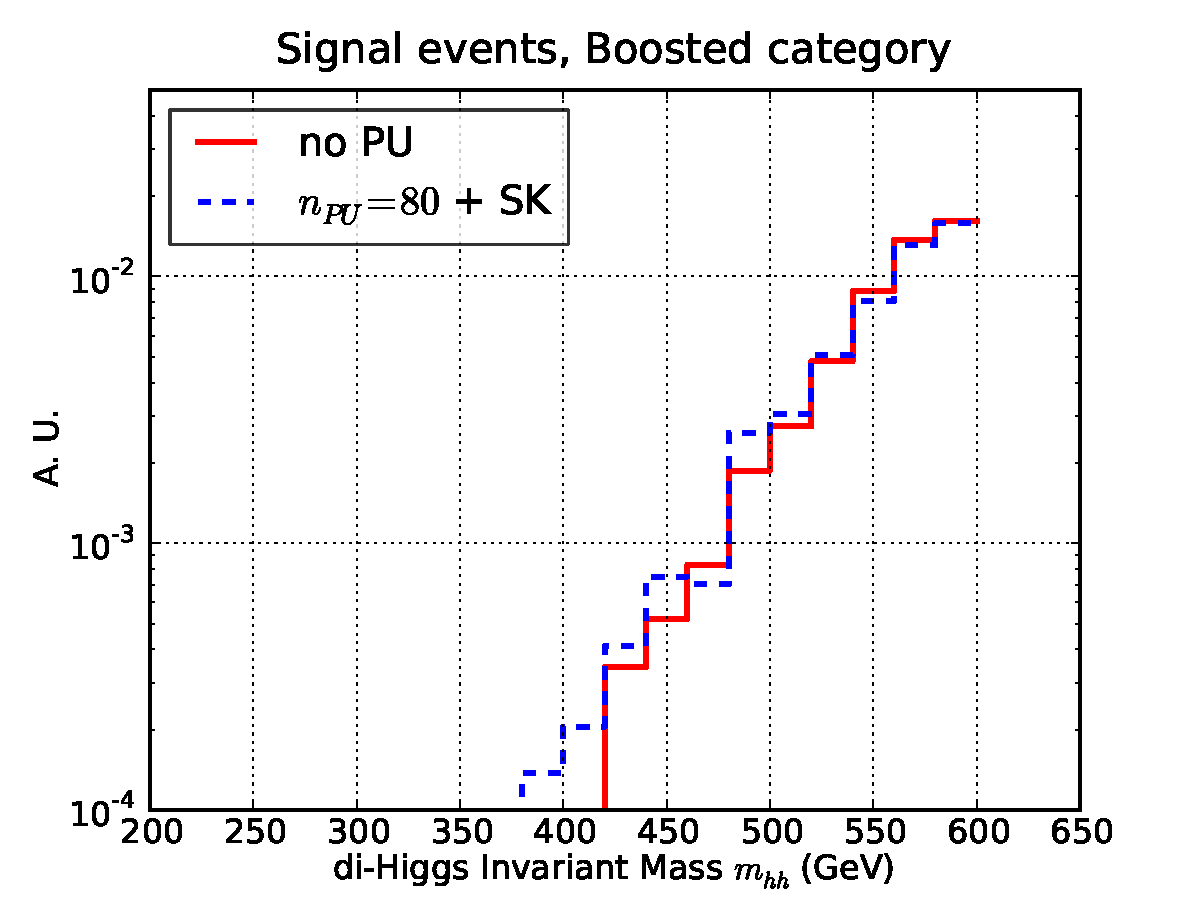
\includegraphics[width=0.49\textwidth]{plots/m_HH_C2_bst_comp.pdf}
  \caption{\small
    Comparison of the transverse momentum $p_T^h$ of the leading
    Higgs candidate (upper plots) and of the invariant mass $m_{hh}$
    of the di-Higgs system (lower plots) in the resolved
    (left plots) and boosted (right plots) categories,
    without PU and with $\la n_{PU}\ra=80$ subtracted with {\tt SoftKiller}.
}
\label{fig:mHH_PU}
\end{center}
\end{figure}
%%%%%%%%%%%%%%%%%%%%%%%

Then we assess the impact of PU in some of the substructure variables
used as input to the MVA in the boosted category.
%
In particular we consider the subjetiness variable,
$\tau_{21}$, and the ratio
of energy correlation functions $D_2^{(\beta)}$,
corresponding to the the leading Higgs candidate.
%
This comparison is illustrated in Fig.~\ref{fig:Substructure_PU}.
%
As can be seen, these substructure variables, which
as demonstrated before carry a very substantial
discrimination power, are relatively unaffected by PU.
%
Therefore, we don't expect a substantial loss of discrimination
power due to PU effects in our analysis.


%%%%%%%%%%%%%%%%%%%%%%%%
\begin{figure}[t]
  \begin{center}
    \vspace{-1cm}
  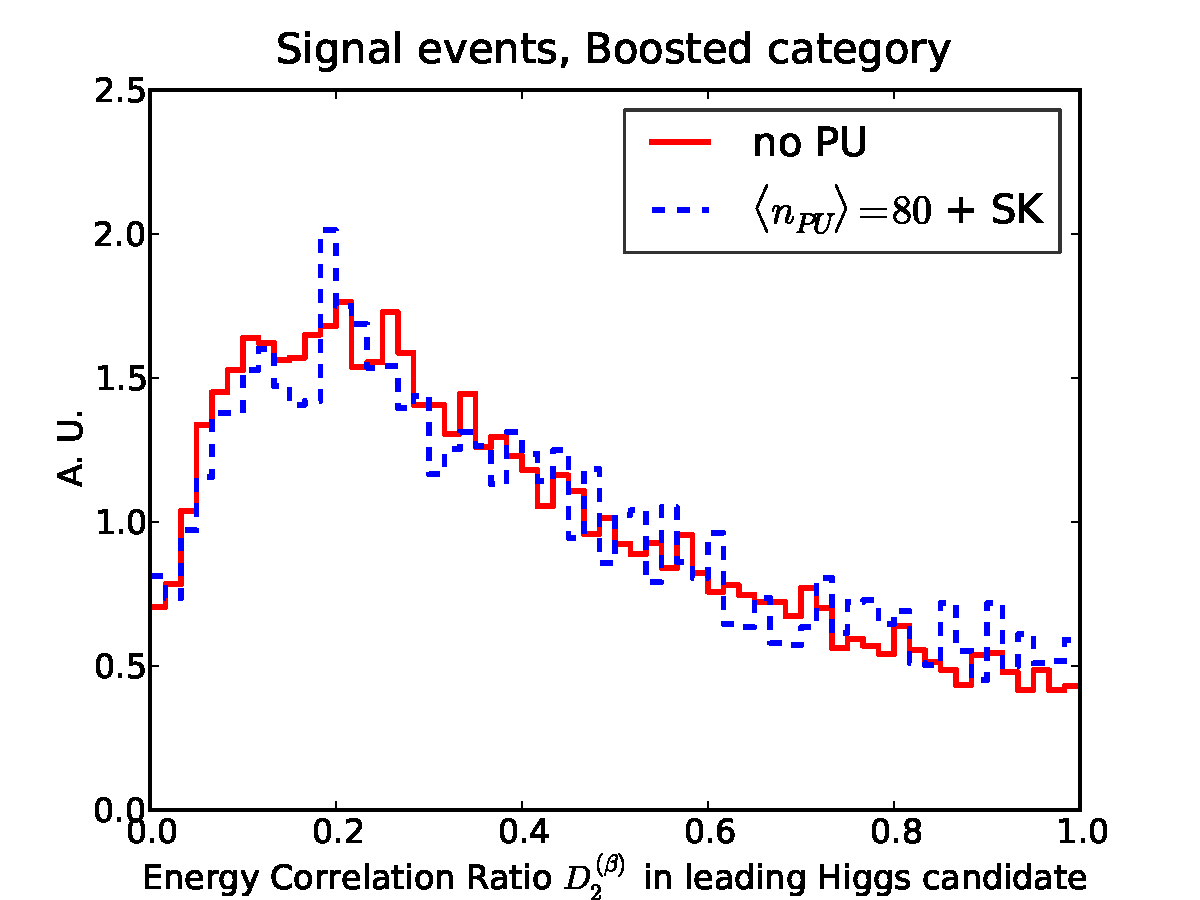
\includegraphics[width=0.49\textwidth]{plots/D2_h0_bst_comp.pdf}
  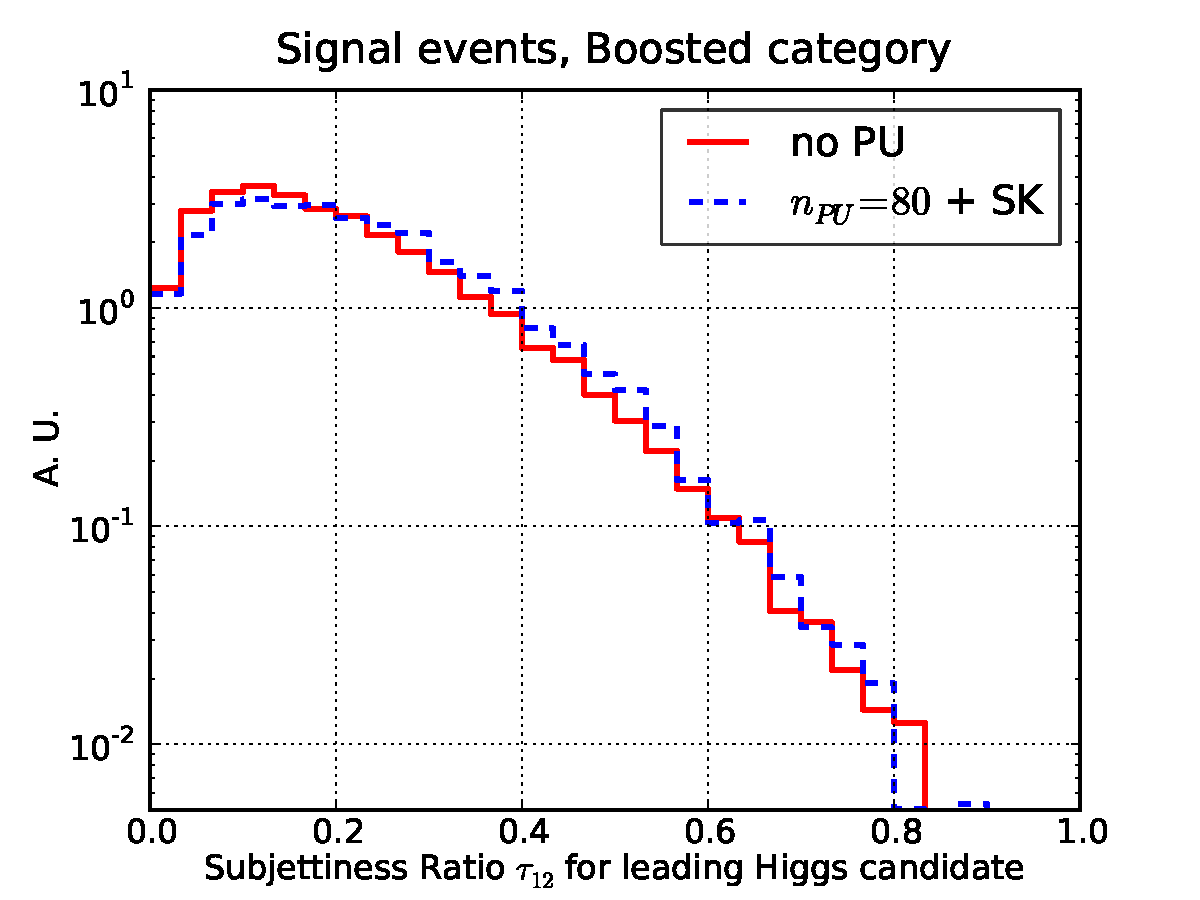
\includegraphics[width=0.49\textwidth]{plots/tau21_h0_bst_comp.pdf}
   \caption{\small
     Comparison of the substructure variables $D_2^{(\beta)}$ (left)
     and $\tau_{21}$ (right)
     for the leading Higgs candidate in the boosted category,
   without PU and with $\la n_{PU}\ra=80$ subtracted with {\tt SoftKiller}.
}
\label{fig:Substructure_PU}
\end{center}
\end{figure}
%%%%%%%%%%%%%%%%%%%%%%%


Up to know we have restricted ourselves to the study of the impact of PU
on signal distributions.
%
We now assess how the signal over background discrimination can be affected
in the presence of realistic PU conditions.

{\bf add plots signal vs background with PU}


\subsection{Signal significance in the presence of PU}

Finally, we revisit how the signal significance after the MVA
is affected by the inclusion of realistic PU effects.


%%%%%%%%%%%%%%%%%%%%%%%%
\begin{figure}[t]
\begin{center}
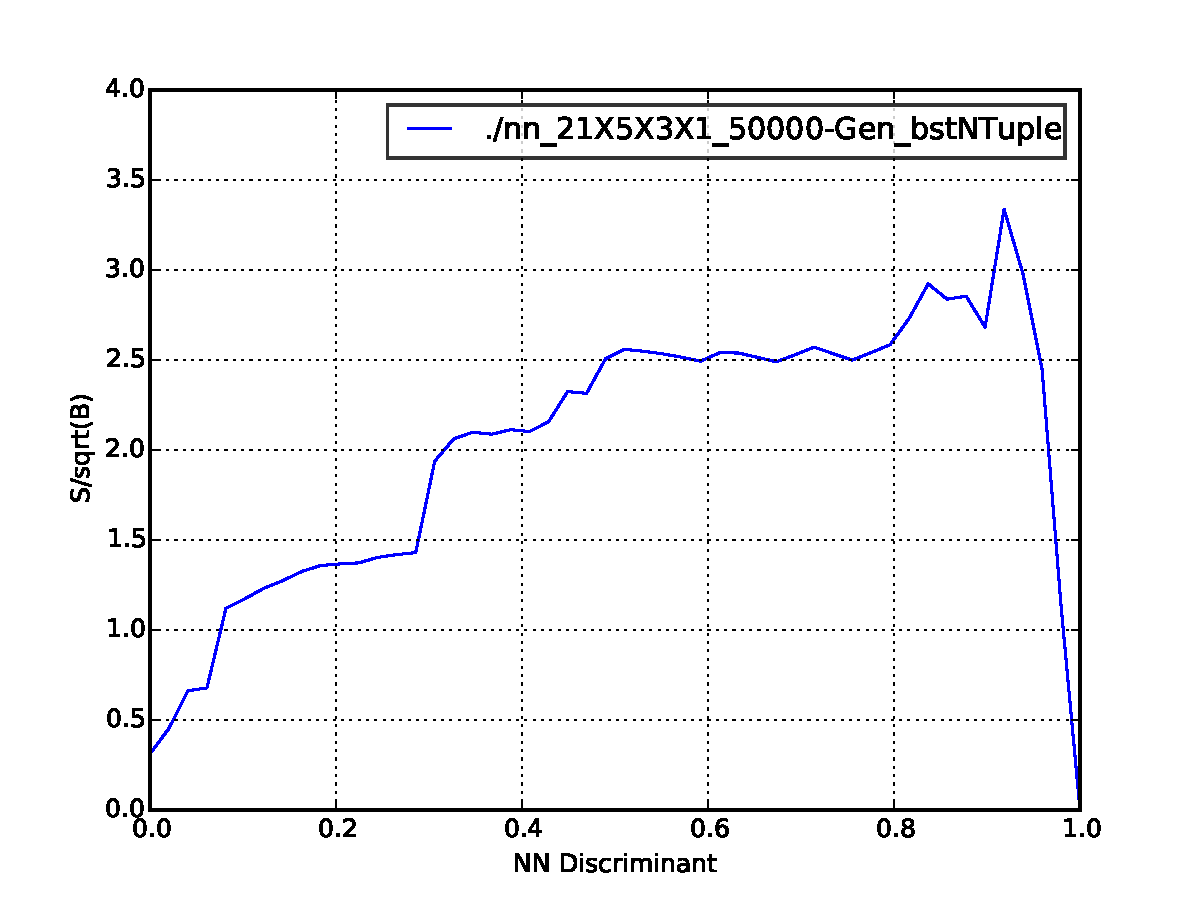
\includegraphics[width=0.48\textwidth]{plots/ssb_pu.pdf}
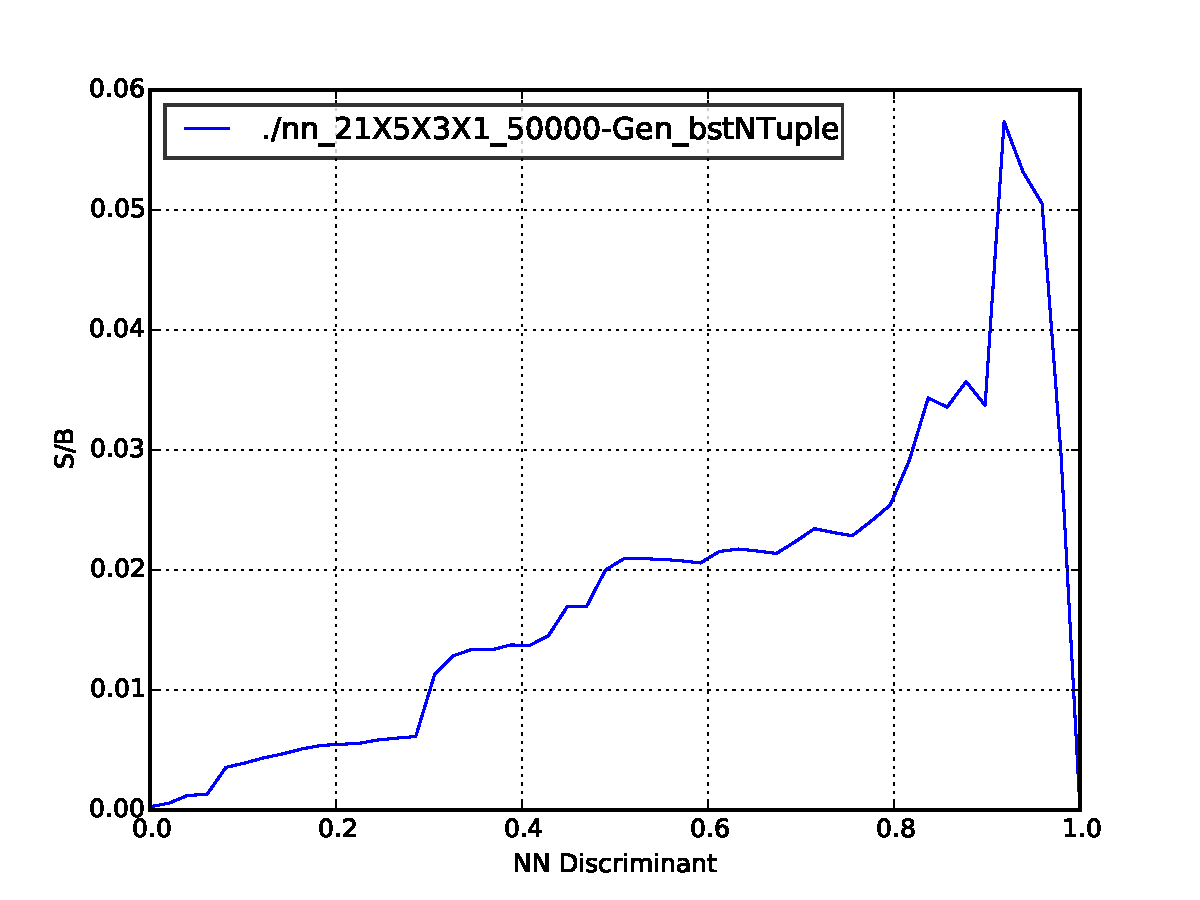
\includegraphics[width=0.48\textwidth]{plots/sb_pu.pdf}
\caption{\small
  Same as Fig.~\ref{fig:sb_mva} this time for the analysis including
  effects of PU, with $\la n_{\rm PU}\ra=150$.
}
\label{fig:sb_mva_pu}
\end{center}
\end{figure}
%%%%%%%%%%%%%%%%%%%%%%%

In Fig.~\ref{fig:sb_mva_pu} we show the signal significance,
$S/\sqrt{B}$, as well as the signal over background ratio,
$S/B$, as a function of the NN discriminant, in the case
of the analysis including the effects of PU
with $\la n_{\rm PU}\ra=150$.
%
The corresponding results in the case without PU were shown in
Fig.~\ref{fig:sb_mva}.
%
As can be seen, the MVA-driven enhancement is robust event in the
presence of PU, and a total signal significance of
almost $S/\sqrt{B}\simeq 3$ is also obtained in this case.
%
Therefore, we conclude that the qualitative results obtained
in the previous section are robust even in the presence
of realistic PU effects.
%
Note that no specific effort has been performed to
optimize PU subtraction (for example by tuning the value
of the patch length $a$ in {\tt SoftKiller}), so there is
certainly still room for improvement.
